%\chapter{開発プロセス}
\section{第3サイクル(9月25日~10月21日)}
第3サイクルは後期が始まった9月25日から10月21日に行われた企業講師とのテレビ会議までとした。本サイクルでは、第2サイクルで見つかった大きな課題の一つである写真を撮る行為にもっとワクワクするような付加価値を加えなければならないこと、そして観光情報をより魅力的に紹介することを課題として活動を進めた。
\par まず我々は、後期が始まって最初の授業で前期を振り返り、もう一度課題を見直した。そして観光情報の表示の仕方について話し合ったとき、Time Out Tokyoが掲載していた「札幌でしかできない50のこと」という記事の存在を知り、それを参考にして木古内で「できること」に着目した情報を表示する形式にすることを決定した。また、それと同時に「アプリからトランプを作ることができたら面白いのではないか」と言う意見が出たため、そのアイデアを膨らませて、撮った写真を利用してカルタという「もの」にする機能を作ることも決定した。カルタという「もの」にする意義は後に説明する。また、この時、テレビ会議までにはできる範囲までは実装を行おうと決め、木古内で「できること」に着目した情報紹介の機能から実装を進めた。具体的に修正した内容を表5.2に、完成した画面イメージと印刷して完成したカルタのサンプルを図5.5、5.6に示す。図の5.5は(a)がメインとなる画面で、この画面から(b)や(c)に遷移することを想定して設計・実装した。それと同時に、アプリ内で紹介する観光スポットの写真を集めるために10月15日にメンバでもう一度木古内へ行き、アプリ内で使用する写真の素材を集めた。詳細は次頁で説明する。パンフレットやWebで掲載されていないような自分たちが見つけた魅力のあるスポットの写真も撮影できた。さらに、本サイクルでまだ決めていなかったアプリのタイトルをメンバ間で話し合った結果、アプリ名を「キーコ紀行」と正式に決定した。
\par 本サイクルではより魅力的に観光情報が表示でき、写真を撮る動機づけとなるアイデアを提案できた。しかし、カルタは50枚を超える紙を印刷しなければいけないため手間がかかるという課題が残った。また、技術面としてはメンバに割り振った部分が独立しており、アプリが部分的にしかできていない状態だったため、早急にメンバ間で開発したものを結合する必要があった。アプリを当時の直近のイベントであったHAKODTEアカデミックリンク2015(以降、アカデミックリンクとする)に開発を間に合わせるようにスケジュールを立てることを決定した。\newpage

\begin{table}[htb]
\centering
\addtocounter{table}{+0}
\caption{第2サイクルから第3サイクルへの変化}
  \begin{tabular}{|l|l|} \hline
    改正前&改正後  \\ \hline 
    \parbox{20zw}{カテゴリごとに写真の一覧を表示} & \parbox{20zw}{写真と同時に紹介文を加えることで木古内で「できること」に着目した情報を表示}\rule[-6mm]{0mm}{14mm} \\  \hline
    \parbox{20zw}{詳細情報を表示してからマップに遷移} &\parbox{20zw}{マップ画面と同時に詳細情報や写真を表示}\\ \hline
    \parbox{20zw}{「フォトストーリ—」という機能でアプリ内で写真を振り返る}\rule[-6mm]{0mm}{14mm} & \parbox{20zw}{カルタという「もの」にして思い出を残す}\\ \hline
  \end{tabular} 
\end{table}

\begin{description}
\item[第2回フィールドワーク]\mbox{}
\end{description}
 このフィールドワークは2015年10月15日に木古内町で行った。フィールドワークの目的は2点で、1点目が「木古内町でできること」を探り発見することであった。この「木古内町でできること」のフォーマットは、ある場所でできることに対して写真と説明文のセットとした。2点目は、その「できること」に対応する紹介写真の撮影であった。目的が明確だったため、第1回フィールドワークのようにメンバごとに交通手段を分担するということはなく、また効率的に情報を収集するために、2つのグループに分かれて行動した。このフィールドワークを行い、計15個の「木古内でできること」のコンテンツを作成した。実際に現地調査を行ってできることを探ったため、コンテンツにフィールドワークでの実際の体験を「何ができるか」という形で反映することができた。特に、旧JR渡島鶴岡駅跡のように観光スポットとしてはあまり有名でなく、Web上でも観光パンフレットでも確認できなかった場所を発見し、紹介できるようになったという点は、現地調査をおこなった利点を上手く活かせた例であった。現地調査からの情報収集は問題なく行えたものの、紹介写真の撮影は写真にグループメンバが映り込んでしまっている等、不十分な部分もあったため、その部分は反省すべき点であった。

\begin{figure}[htbp]
  \begin{center}
    \begin{tabular}{c}

      % 1
      \begin{minipage}{0.33\hsize}
        \begin{center}
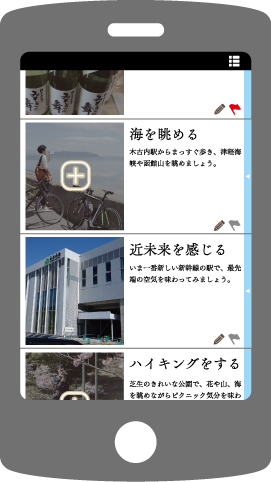
\includegraphics[width=4cm, bb=0 0 320 552]{appIdea1.png}
          \hspace{1cm} (a)観光スポットの紹介
        \end{center}
      \end{minipage}

      % 2
      \begin{minipage}{0.33\hsize}
        \begin{center}
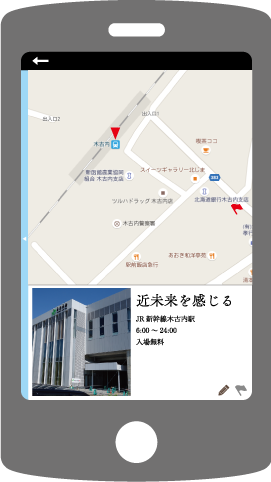
\includegraphics[width=4cm, bb=0 0 321 547]{appIdea2.png}
          \hspace{1cm} (b)詳細情報の表示
        \end{center}
      \end{minipage}

      % 3
      \begin{minipage}{0.33\hsize}
        \begin{center}
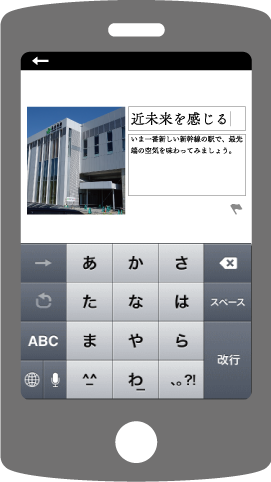
\includegraphics[width=4cm, bb=0 0 320 548]{appIdea3.png}
          \hspace{1cm} (c)紹介文の編集
        \end{center}
      \end{minipage}

    \end{tabular}
    \caption{第3サイクルの完成画面イメージ}
    \label{fig:lena}
  \end{center}
\end{figure}

\begin{description}
\item[カルタにする意義]\mbox{}
 \begin{itemize}
 \item iPhoneという小さい画面の中で振り返る必要が無い。
 \item 写真だけでなく、言葉と一セットになる形式を持っているため、より強く思い出を振り返ることができる。
 \item 実際に「もの」という形にすることで長く保管されやすい。
 \item 遊びながら思い出を振り返ることができる。
 \end{itemize}
\item[本サイクルの提案に対するレビュー内容]\mbox{}
 \begin{itemize}
 \item 「できること」に着目したことによって「どこに行こう?」から「ここに行きたい!」に近づいた。
 \item 実際に印刷する段階まで行ってほしい。
 \item 類似サービス(例えば富士フィルム株式会社のフォトブック)の観光版のフォトブックとして作ってみるのは良い。
 \item ニーズはあると思う。
 \item 図5.6のようなカルタとは違う別の何かにした方が良い。手間がかかるから。
 \item 写真のプロトタイプを作って木古内の関係者に提案するのも良い。まずは見てもらうことが重要。
 \end{itemize}
\end{description}

\begin{figure}[htbp]
  \begin{center}
    \begin{tabular}{c}

      % 1
      \begin{minipage}{0.33\hsize}
        \begin{center}
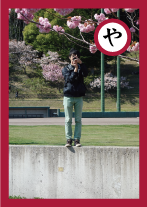
\includegraphics[width=4cm, bb=0 0 320 552]{karuta1.png}
        \end{center}
      \end{minipage}

      % 2
      \begin{minipage}{0.33\hsize}
        \begin{center}
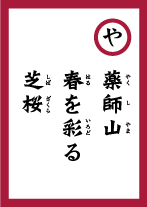
\includegraphics[width=4cm, bb=0 0 321 547]{karuta3.png}
        \end{center}
      \end{minipage}

      % 3
      \begin{minipage}{0.33\hsize}
        \begin{center}
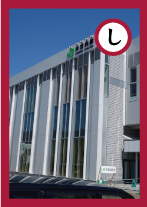
\includegraphics[width=4cm, bb=0 0 320 548]{karuta2.png}
        \end{center}
      \end{minipage}

    \end{tabular}
  \end{center}
\addtocounter{figure}{+0}
 \caption{カルタの完成サンプル}
\end{figure}

\bunseki{山川拓也}